\documentclass[a4paper,10pt]{article}

%\usepackage[utf8]{inputenc}
\usepackage{graphicx}
\usepackage{url}
\usepackage{float}
\usepackage{times}
\usepackage{multirow}
\usepackage{listings}
\usepackage{times}
\usepackage{paralist}
\usepackage{epsfig}
\usepackage{subfigure}
\usepackage[hypertex]{hyperref}
\usepackage{subfigure}
\usepackage{color}
\usepackage{ifpdf}
\usepackage{wrapfig}

\usepackage{texdraw}
\usepackage{epsf}
\usepackage{array}
\usepackage{cite}
\usepackage{enumitem}
\usepackage{verbatim}
\usepackage{setspace}
\sloppy
\usepackage{geometry}



\newcommand{\I}[1]{\textit{#1}}
\newcommand{\B}[1]{\textbf{#1}}
\newcommand{\BI}[1]{\textbf{\textit{#1}}}
\newcommand{\T}[1]{\texttt{#1}}
\newcommand{\dctf}{dC$_{25}$ }
\newcommand{\dctfnsp}{dC$_{25}$}
\newcommand{\atf}{A$_{25}$ }
\newcommand{\dco}{dC$_{1}$ }
\newcommand{\atfnsp}{A$_{25}$}
\newcommand{\dconsp}{dC$_{1}$}
\newcommand{\aonsp}{A$_{1}$}
\newcommand{\ao}{A$_{1}$ }
\newcommand{\ato}{A$_{1}$ }
\newcommand{\ahl}{$\alpha$HL }
\newcommand{\ahlnsp}{$\alpha$HL}
\newcommand{\prim}{$^{\prime}$ }
\newcommand{\primnsp}{$^{\prime}$}


\pdfpagewidth 8.5in
\pdfpageheight 11in 

\setlength\topmargin{0in}
\setlength\headheight{0in}
\setlength\headsep{0in}
\setlength\textheight{9in}
\setlength\textwidth{6.5in}
\setlength\oddsidemargin{0in}
\setlength\evensidemargin{0in}
\setlength\parindent{0.1in}
\setlength\parskip{0.25em}

\ifpdf
 \DeclareGraphicsExtensions{.pdf, .jpg, .png}
\else
 \DeclareGraphicsExtensions{.eps, .ps}
\fi

\newcommand{\up}{\vspace*{-1em}}
\newcommand{\upp}{\vspace*{-0.5em}}
\newcommand{\tc}{$T_c$ }
\newcommand{\ttc} {TTC}
\newcommand{\tcc}{TCC}

\newcommand{\jha}[1]{ {\textcolor{red} { ***Jha: #1 }}}

\begin{document}
\title{\LARGE % Investigating Scale-Out Performance of 
% Loosely-Coupled Simulations Using Multiple Distributed Resources on the TeraGrid.
  Progress Report for TeraGrid Allocation TG-MCB090174}

% \author{Principal Investigator: Shantenu Jha$^{1,2}$ \\
% Co-Principal Investigator: Joohyun Kim$^{1}$ \\ 
% Co-Principal Investigator: Yaakoub El KhNSFamra$^{3}$\\\
%    \small{\emph{$^{1}$Center for Computation \& Technology, Louisiana State University, Baton Rouge, 
% USA}}
% \\
%   \small{\emph{$^{2}$Department of Computer Science, Louisiana State
%       University, Baton Rouge, USA}}
% \\
%   \small{\emph{$^{3}$Texas Advanced Computing Center TACC, University of Texas, Austin, USA}}}

\newif\ifdraft
\drafttrue
\ifdraft
\newcommand{\amnote}[1]{ {\textcolor{magenta} { ***AM: #1c }}}
\newcommand{\jhanote}[1]{ {\textcolor{red} { ***SJ: #1 }}}
\newcommand{\michaelnote}[1]{ {\textcolor{blue} { ***MM: #1 }}}
\newcommand{\yyenote}[1]{ {\textcolor{green} { ***YYE: #1 }}}
\else
\newcommand{\amnote}[1]{}
\newcommand{\jhanote}[1]{}
\newcommand{\michaelnote}[1]{ {\textcolor{blue} { ***MM: #1 }}}
\newcommand{\yyenote}[1]{ {}}
\fi

%\date{15 July 2010}

\date{}

\maketitle
\up\up\up\up


%\section{Results From Prior Awards}

% \jhanote{This should list out (i) prior awards and what they were for, (ii) scientific progress and understanding that arose and (ii) publications as a result of prior awards.}

% \jhanote{Yaakoub/Joohyun: Our award/project number for last years TRAC is MCB090174.
%   Please mention resource usage statistics, be sure to mention that we've used 100\% well before
%   the expiry. Mention allocation swapping between machines}

% \jhanote{Publications arising from clast TRAC: (i) Project 1: JCTC and a publication on ABF are in the works; (ii) Riboswtich -- in addition to NAR, we have ECMLS and others (Joohyun to fix), (iii) UCL is listed in prior.tex so ok, (iv) Project 4, TeraGrid-talk, DEISA Interop talk, and publication in process, but also reference Cybertools publications -- ccgrid and others}


This group has multiple publications arising from earlier TRAC Awards. Initial results from Project 1 supported by the most recent TRAC award to PI Jha (MCB090174) was selected as the cover article of a leading scientific journal~\cite{jctc_cover}.  \begin{wrapfigure}{r}{0.28\textwidth}
 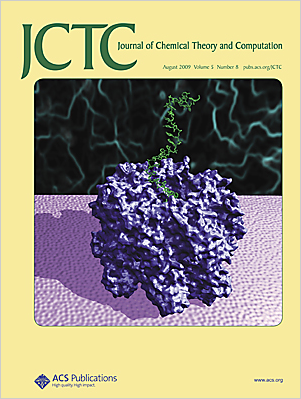
\includegraphics[width=0.28\textwidth]{jctc_cover2.png}
 \caption{\footnotesize JCTC Cover Article}
 \label{cover}
\end{wrapfigure}
Using previous TRAC allocations, we have performed all-atom MD simulations for the SAM-I riboswtich study.  We have reported our scientific results in recent conferences~\cite{ecmls10}, as well a recently published journal article in the prestigious Nucleic Acids Research\cite{SAM-I-NAR2009} (Impact Factor $>$ 7.0). On the basis of these publications, we have enhanced our scope by expanding our interests \& simulations to other riboswitches, such as TPP riboswitches and recurrent RNA structural motifs such as K-turn, towards a comprehensive understanding of the mechanisms of SAM riboswitches.  Also, we added the complementary computational approaches such as RNA secondary structure prediction in addition to all-atom MD simulations, and our initial effort was presented in the workshop, "Emerging Computational Methods for the Life Sciences" held in conjunction with ACM HPDC 2010\cite{ecmls10}.

Previously we have used TeraGrid resources to conduct a binding affinity study of the protease inhibitor saquinavir with G48V and L90M containing mutatants which showed good agreement with experiment \cite{Stoica2008}. % uring SuperComputing 2007 we used
Using Lonestar (TG allocation number TG-ASC070019T) to expand this work by running 10ns-long simulations on 5 different HIV protease systems bound to 5 different FDA-approved drugs: amprenavir, indinavir, lopinavir, ritonavir, and saquinavir. We compared our binding energy results for each of the 5 protease genotypes in the MDR set to experimental values published in \cite{Ohtaka2003}. Our results showed varying correlations to experimental trends, with the 5 ritonavir systems showing good correlation to experimental whilst the 5 saquinavir systems showed poor correlation. In light of these results further work was done both on Lonestar (TG allocation numbers TG-ASC070019T and TG-DMR070014N) and more recently Ranger (TG allocation numbers A-rfUser1 and TG-ASC090009) to determine whether repeating the study as an ensemble of MD models would improve correlations. The results showed significantly improved correlations and have led us to refine our simulation protocol and reparameterise a number of inhibitors. An article focussed primarily on our work on the lopinavir bound system has recently been accepted for publication \cite{Sadiq2010}.

In addition to this we have performed a study into the comparative dynamics of different liganded forms of reverse transcriptase, concluding that the binding of the inhibitors efavirenz and nevirapine alter the motions of the catalytically important fingers domain of RT and that these motions are uncorrelated to fluctuations in the drug binding energy (as yet unpublished). We also performed preliminary investigations into the efficacy of the ensemble methodology for calculating binding affinities on NVP bound systems, again concluding that the convergence properties are improved over single trajectory. These results also allowed us to differentiate binding affinity of the L100I and L100I/K103N sequences from the wildtype using simulations of the ligand bound enzyme alone which indicates that they do not significantly affect the creation of the binding pocket. All this work was performed using Ranger. 

These simulations were orchestrated using our automated simulation tool, the Binding Affinity Calculator (BAC), which makes use of AHE \cite{coveney2007,zasada2009} to deploy and run simulations and then retrieve data. Two papers describing this tool and its potential use as a clinical support tool have been published\cite{Sadiq2008, Sadiq2008a}. The BAC allows us to distribute the simulation and analysis sections of our workflow over a number of geographically disparate locations. The mutation and hydration of crystal structure based models takes place on local resources at UCL, using the AMBER software suite, while the actual simulations can be performed in NAMD either on TeraGrid or UKNational Grid Service (NGS) computers and/or EU DEISA grid. The final analysis of the resultant trajectories, either on local recources or the NGS, is performed using the AMBER MD suite of codes. In the last year, BAC has been extended to allow the simulation of the epidermal growth factor receptor (EGFR) and the molecular dynamics code GROMACS \cite{Hess2008}. This new functionality has facilitated a study of the binding of three inhibitors (AEE788, AFN941 and getfitinib) bound to EGFR, performed on Ranger.

In the area of bio-minerals our previous simulations have utilized periodic boundaries on the clay sheets, allowing a simulation cell to represent an infinite clay platelet \cite{JPCC_2007,Thyveetil,Thyveetil_JACS, Soft_Matter1}. These large-scale, fully atomistic simulations, approached the size of a physically realistic platelet. From this, we were able to calculate mesoscopic and macroscopic properties directly from molecular dynamics simulations in the absence of finite-size effects of both clay nanocomposites\cite{JPCC_2007,Thyveetil, Soft_Matter1} and bio-composites~\cite{Thyveetil_JACS}.  Using resources from TG-ASC070019T we extended these simulations to calculate the mechanical response of poly(ethylene oxide) polymer-clay nanocomposites, separating the response into contributions from the polymer and clay mineral layer~\cite{Soft_Matter1}. This separation technique allowed us to determine how the clay-polymer elastic properties change with distance from the clay surface. This is the first time the effect of mineral layers on the elastic modulus of polymeric materials in the vicinity of a mineral surface has been calculated. This result is a vital first step to understanding the enhancement mechanism of nanocomposites and the role of the very large surface area of the clay mineral layer on the surrounding medium.  We have also examined the mechanisms by which clay mineral layers buckle in clay-polymer nanocomposites under compressive stress. We find that a clay sheet remains stable in a flat state until a critical compressive strain is reached, at which point it buckles, and regains its uncompressed area. Over this buckling transition, the Poisson ratio of the clay sheets turns negative, a property which has been predicted for 2-dimensional sheets ~\cite{Soft_Matter2}. This is the first time such behaviour has been seen in a molecular simulation of mineral layers. The large scale allowing us to probe large buckling wavelengths that are inhibited in smaller scale simulation.
% To simulate a realistically sized clay platelet required very large scale simulations, made possible using the resources available via the LRAC allocation.

We have also used previous TRAC allocation for CO$_2$ sequestration studies and reservoir characterization studies. These studies were composed of running an ensemble of independent simulations followed by an anaylsis step, and iterating until a termination criteria is met.  Since the simulations are independent, they can be distributed across TeraGrid resources, with a sufficiently abstract and sophisticated workflow manager.  We have begun developing an rudimentary distributed autonomic framework -- Lazarus ~\cite{gmac}, using which we are able to select multiple TeraGrid machines concurrently, dynamically optimize the work-load and gain deep insights. This is a natural continuation of our award winning work in 2008 (TeraGrid 2008 Performance Challenge Award)~\footnote{\url{http://www.cct.lsu.edu/~sjha/select_publications/tg08-performance-award.pdf}}. Beside the obvious science results ~\cite{TG10yye00}, we learned a great deal about scale-out behavior and management of ensembles of large scale simulations, the need for fault tolerance and autonomic behavior, as well as the promising possibilities of combining Grid and Cloud environments. This work has resulted in several publications \cite{Cloud1,Cloud2,MSEScience,TG10yye00} and presentations as well as a Masters degree~\cite{Elkhamra2009}.




\newpage

\bibliographystyle{unsrt}


%\begin{thebibliography}{10}

\bibitem{jarz}
C. Jarzynski. Phys. Rev. Lett., 78(14):2690�2693, 1997.

\bibitem{namd}
J. Philips et al. Journal of Computational Chemistry. 26, 1781-1802, 2005.

\bibitem{akeson}
M. Akeson et al. Biophys. J., 77(6):3227�3233, 1999.

\bibitem{foloppe}
N. Foloppe et al. Drug Discovery Today. 11, 1019-1027, 2006.

\bibitem{mandal}
M. Mandal et al. Nat Rev Mol Cell Biol. 5(6), 451-63, 2004.

\bibitem{brooke}
B. A. M. McDaniel et al. Proc. Natl. Acad. Sci. U.S.A. 100, 3083-3088, 2003.

\bibitem{SAM-I-NAR2009}
W.~Huang, J.~Kim, S.~Jha, and F.~Aboul-ela.
\newblock A mechanism for s-adenosyl methionine assisted formation of a
  riboswitch conformation: A small molecule with a strong arm.
\newblock {\em Nucleic Acid Research}, submitted.

\bibitem{montange}
R. K. Montange et al. Nature. 255, 1172-1175, 2006.

\bibitem{alberto}
P. Alberto, et al. Biophysical Journal. 92, 3817-3829, 2007.

\bibitem{wang}
J. Wang et al. Journal of Molecular Graphics and Modelling , 25, 247260, 2006,.

\bibitem{moe}
Molecular Operating Environment (MOE 2007.9), Chemical Computing Group (CCG).

\bibitem{saga_url}
The Simple API for Grid Applications, http://saga.cct.lsu.edu.

\bibitem{saga_escience07}
S.~Jha, H.~Kaiser, Y.~El Khamra, and O.~Weidner.
\newblock Design and implementation of network performance aware applications
  using saga and cactus.
\newblock In {\em Accepted for 3rd IEEE Conference on eScience2007 and Grid
  Computing, Bangalore, India.}, 2007.

\bibitem{gmac}
Y.~El Khamra and S.~Jha.
\newblock Title: {Developing Autonomic Distributed Scientific Applications: A
  Case Study From History Matching Using Ensemble Kalman-Filters}.
\newblock In {\em Sixth International Conference on Autonomic Computing, 2009.
  ICAC '09 (Barcelona)}. IEEE, 2009.

\bibitem{REMD-PhilTranA2009}
A.~Luckow, S.~Jha, J.~Kim, A.~Merzky, and B.~Schnor.
\newblock Adaptive distributed replica-exchane simulations.
\newblock {\em Phil. Tran. A}, 367:2595, 2009.

\bibitem{saga_loosely_coupled}
Developing Scientific Applications With Loosely-Coupled Sub-Tasks, accepted
  International Conference on Computational Science (ICCS), in Baton Rouge, Jan
  2009.

\bibitem{teragrid08}
S.~Jha, K.~Hartmut, Y.~El Khamra, and O.~Weidner.
\newblock Developing adaptive scientific applications with hard to predict
  runtime resource requirements with saga.
\newblock In {\em Proceedings of the TeraGrid 2008 Conference}, 2008.

\bibitem{saga_data_intensive}
Programming Abstraction for Data Intensive Computing on Clouds and Grids,
  accepted at Intl. Workshop on Cloud Computing, 2009, in conjunction with
  CCGrid2009. Draft at:
  {\href{http://www.cct.lsu.edu/~sjha/publications/saga\_data\_intensive.pdf}{%
\url{http://www.cct.lsu.edu/~sjha/publications/saga\_data\_intensive.pdf}}}.

\bibitem{saga_grid_cloud}
Application Level Interoperability between Clouds and Grids accepted for First
  International Workshop on Grids and Clouds, held in conjunction with
  Conference on Grid and Pervasive Computing, Geneva, 2009. Draft at: \\
  \url{http://www.cct.lsu.edu/~sjha/publications/saga\_cloud\_interop.pdf}.

\bibitem{GeoRPT}
D.~J.~DePaolo et~al.
\newblock Basic research needs for geosciences:facilitating 21st century energy
  systems.
\newblock {\em Office of Basic Energy Sciences, U.S. Department of Energy},
  2007.

\bibitem{EORBook}
D.~W. Green and G.~P. Willhite.
\newblock {\em Enhanced Oil Recovery}, volume~6.
\newblock 1998.

\bibitem{Luigi}
L.~Marini.
\newblock {\em Geological Sequestration of Carbon Dioxide, Volume 11:
  Thermodynamics, Kinetics, and Reaction Path Modeling (Developments in
  Geochemistry)}, volume~11.
\newblock 2007.

\bibitem{KalmanPaper}
R.~E. Kalman.
\newblock A new approach to linear filtering and prediction problems.

\bibitem{DO2007}
Y.~Gu and D.~S. Oliver.
\newblock An iterative ensemble kalman filter for multiphase fluid flow data
  assimilation.
\newblock {\em SPE Journal}, 12(4):438--446, 2007.

\bibitem{LiEnKF07}
X.~Li, C.~White, Z.~Lei, and G.~Allen.
\newblock Reservoir model updating by ensemble kalman filter-practical
  approaches using grid computing technology.
\newblock In {\em Petroleum Geostatistics 2007}, Cascais,Portugal, August 2007.

\bibitem{DO2006}
Y.~Gu and D.~S. Oliver.
\newblock The ensemble kalman filter for continuous updating of reservoir
  simulation models.
\newblock {\em Journal of Engineering Resources Technology}, 128(1):79--87,
  2006.

\bibitem{interop_url}
TeraGrid-LONI Interoperabilty Project, {\it A Science-Driven Project Using
  Advanced CyberInfrastructure funded by NSF via a HPCOPS award to LONI},
  {\url{http://www.teragridforum.org/mediawiki/index.php?title=LONI-TeraGrid-D%
EISA\_Interoperabilty\_Project}}.

% \end{thebibliography}
% \begin{thebibliography}{10}

\bibitem{zasada2009}
P.~V. Coveney and S.~J. Zasada.
\newblock Virtualizing access to scientific applications with the {Application
  Hosting Environment}.
\newblock {\em Comp. Phys. Comm.}, 180(12):2513--2525, 2009.

\bibitem{coveney2007}
P.~V. Coveney, R.~S. Saksena, S.~J. Zasada, M.~McKeown, and S.~Pickles.
\newblock The application hosting environment: Lightweight middleware for
  grid-based computational science.
\newblock {\em Comp. Phys. Comm.}, 176:406--418, 2007.

\bibitem{chaos-book}
P.~Cvitanovi{\'{c}}, R.~Artuso, R.~Mainieri, G.~Tanner, G.~Vattay, N.~Whelan,
  and A.~Wirzba.
\newblock {\em Chaos: Classical and Quantum (http://www.chaosbook.org/)}.
\newblock Niels Bohr Institute, Copenhagen, 2005.

\bibitem{artuso}
R.~Artuso, E.~Aurell, and P.~Cvitanovi{\'{c}}.
\newblock Recycling of strange sets \uppercase{i}: cycle expansions.
\newblock {\em Nonlinearity}, 3:325--359, 1998.

\bibitem{bohr-jensen}
T.~Bohr, M.~H. Jensen, G.~Paladin, and A.~Vulpiani.
\newblock {\em Dynamical Systems Approach to Turbulence (Cambridge Nonlinear
  Science Series)}.
\newblock Cambridge University Press, 1998.

\bibitem{lan-cvitanovic}
Y.~Lan and P.~Cvitanovi\ifmmode~\acute{c}\else \'{c}\fi{}.
\newblock Variational method for finding periodic orbits in a general flow.
\newblock {\em Phys. Rev. E}, 69(1):016217, 2004.

\bibitem{Comput-HYPO4D}
L.~Fazendeiro, B.~M. Boghosian, P.~V. Coveney, and J.~L{\"{a}}tt.
\newblock Unstable periodic orbits in turbulent hydrodynamics.
\newblock {\em Submitted to the Journal of Computational Science}, 2009.

\bibitem{draft-bogh-tam2}
B.~M. Boghosian, P.~V. Coveney, L.~Fazendeiro, J.~L{\"{a}}tt, J.~Tam, and
  H.~Tang.
\newblock A computational program for the dynamical systems approach to
  turbulence.
\newblock {\em Submitted to Journal of Computational Science}, 2010.

\bibitem{saksenapetascale}
R.~S. Saksena, B.~M. Boghosian, L.~Fazendeiro, O.~A. Kenway, S.~Manos,
  M.~Mazzeo, S.~K. Sadiq, J.~L. Suter, D.~Wright, and P.~V. Coveney.
\newblock Real science at the petascale.
\newblock {\em Phil. Trans. R. Soc. A}, 367(1897):2557--2571, 2009.

\bibitem{viswanath2007}
D.~Viswanath.
\newblock Recurrent motions within plane {Couette} turbulence.
\newblock {\em J. Fluid Mech.}, 580:339--358, 2007.

\bibitem{gibson2008}
J.~F. Gibson, J.~Halcrow, and P.~Cvitanovi\'{c}.
\newblock Visualizing the geometry of state space in plane couette flow.
\newblock {\em J. Fluid Mech.}, 611:107--130, 2008.

\bibitem{dennis1996}
J.~E. Dennis~Jr and R.~B. Schnabel.
\newblock Numerical methods for unconstrained optimization and nonlinear
  equations.
\newblock {\em SIAM}, 1996.

\bibitem{doctors2009}
G.~M. Doctors, M.~D. Mazzeo, and P.~V. Coveney.
\newblock {A computationally efficient method for simulatioon of fluid flow in
  elastic pipes in toand three dimensions}.
\newblock {\em Submitted to Computer Physics Communications}, 2009.

\bibitem{mazzeo2010}
M.~D. Mazzeo, S.~Manos, and P.~V. Coveney.
\newblock {In situ ray tracing and computational steering for interactive blood
  flow simulation}.
\newblock {\em Computer Physics Communications}, 181:355--370, 2010.

\bibitem{manostg08}
S.~Manos, S.~Zasada, M.~D. Mazzeo, R.~Haines, G.~Doctors, S.~Brew, R.~Pinning,
  J.~Brooke, and P.~V. Coveney.
\newblock {Patient specific whole cerebral blood flow simulation: A future role
  in surgical treatment for neurovascular pathologies}.
\newblock {\em Winner of 'Transformational Science Challenge' award at TeraGrid
  2008}, 2008.

\bibitem{manoshpdc08}
S.~Manos, M.~Mazzeo, O.~Kenway, P.~V. Coveney, N.~T. Karonis, and B.~Toonen.
\newblock Distributed {MPI} cross-site run performance using mpig.
\newblock In {\em HPDC '08: Proceedings of the 17th international symposium on
  High performance distributed computing}, pages 229--230, New York, NY, USA,
  2008. ACM.

\bibitem{manosctw08}
S.~Manos, S.~Zasada, and P.~V. Coveney.
\newblock {Life or Death Decision-making: The Medical Case for Large-scale,
  On-demand Grid Computing}.
\newblock {\em CTWatch Quarterly}, 4(1), 2008.

\bibitem{mazzeo2008}
M.~D. Mazzeo and P.~V. Coveney.
\newblock {HemeLB: A high performance parallel lattice-Boltzmann code for large
  scale fluid flow in complex geometries}.
\newblock {\em Computer Physics Communications}, 178(12):894--914, 2008.

\bibitem{saksena2008}
R.~S. Saksena and P.~V. Coveney.
\newblock Self-assembly of ternary cubic, hexagonal, and lamellar mesophases
  using the lattice-{B}oltzmann kinetic method.
\newblock {\em J. Phys. Chem. B}, 112(10):2950 -- 2957, 2008.

\bibitem{harting2004_2}
J.~Harting, Chin. J., M.~Venturoli, and P.~V. Coveney.
\newblock Large-scale grid-enabled lattice-boltzmann simulations of complex
  fluid flow in porous media and under shear.
\newblock {\em Phil. Trans. R. Soc. Lond. A}, 362:1703--1722, 2004.
\newblock there is an updated publication from 2005.

\bibitem{cates2008sm}
M.~E. Cates and P.~S. Clegg.
\newblock Bijels: {A} new class of soft materials.
\newblock {\em Soft Matter}, 4:2132--2138, 2008.

\bibitem{saksena2009_2}
R.~S. Saksena and P.~V. Coveney.
\newblock Shear rheology of amphiphilic cubic liquid crystals from large-scale
  kinetic lattice-boltzmann simulations.
\newblock {\em Soft Matter}, 5:4446--4463, 2009.

\bibitem{saksena1024}
R.~S. Saksena and P.~V. Coveney.
\newblock Defect texture dynamics under couette flow in amphiphilic liquid
  crystals from large-scale lattice-boltzmann simulations. {Preprint} 2010.

\bibitem{saksena2009}
R.~S. Saksena and P.~V. Coveney.
\newblock Rheological response and dynamics of an amphiphilic diamond phase.
\newblock {\em Proc. R. Soc. A}, 465:1977--2002, 2009.

\bibitem{saksenaahm09}
R.~S. Saksena, S.~J. Zasada, M.~D. Mazzeo, and P.~V. Coveney.
\newblock Petascale lattice-{B}oltzmann simulations of amphiphilic cubic liquid
  crystals. {Preprint 2010.}

\bibitem{bmb2005}
B.~M. Boghosian and P.~V. Coveney.
\newblock Scientific applications of grid computing.
\newblock {\em Computing in Science and Engineering}, 7(5):10--13, 2005.

\bibitem{blake-coveney-clarke-pickles-05}
R.~J. Blake, P.~V. Coveney, P.~Clarke, and S.~M. Pickles.
\newblock {\em Scientific Programming}, 13:1--17, 2005.

\bibitem{mckeown_ptrsla05}
R.~Haines, M.~McKeown, S.~M. Pickles, R.~L. Pinning, A.~R. Porter, and
  M.~Riding.
\newblock The service architecture of the teragyrid experiment.
\newblock {\em Phil. Trans. R. Soc. A}, 363:1743--1755, 2005.

\bibitem{hector}
{h}ttp://www.hector.ac.uk.

\bibitem{jens}
Private Communication. {Also see
  {www.hc-europa.eu/files/registrationTAM/6-Florian\%20JANOSCHEK.pdf}}.

\bibitem{JPCC_2007}
J.~L.~Suter \emph{et al}.
\newblock Large-scale molecular dynamics study of montmorillonite clay:
  Emergence of undulatory fluctuations and determination of material
  properties.
\newblock {\em J. Phys. Chem. C}, 111(23):8248--8259, 2007.

\bibitem{Franchi}
M.~Franchi, J.~P. Ferris, and E.~Gallori.
\newblock Cations as mediators of the adsorption of nucleic acids on clay
  surfaces in prebiotic environments.
\newblock {\em {Origins of Life and Evolution of the Biosphere}}, {33}:{1--16},
  {2003}.

\bibitem{Huang}
W. H. Huang and J. P. Ferris.
\newblock One-step, regioselective synthesis of up to 50-mers of {RNA}
  oligomers by montmorillonite catalysis.
\newblock {\em {Journal of the American Chemical Society}}, {128}:{8914--8919},
  {2006}.

\bibitem{understanding}
B.~Chen, J.~R.~G. Evans, H.~C. Greenwell, P.~Boulet, P.~V. Coveney, A.~A.
  Bowden, and A.~Whiting.
\newblock A critical appraisal of polymer-clay nanocomposites.
\newblock {\em Chem. Soc. Rev.}, 37:568--594, 2007.

\bibitem{Thyveetil}
M.-A. Thyveetil, P.~V. Coveney, J.~L. Suter, and H.~C. Greenwell.
\newblock Emergence of undulations and determination of materials properties in
  large-scale molecular dynamics simulation of layered double hydroxides.
\newblock {\em Chem. Mater.}, 19(23):5510--5523, 2007.

\bibitem{Thyveetil_JACS}
M.-A. Thyveetil, P.V. Coveney, H.~C. Greenwell, and J.~L. Suter.
\newblock Computer simulation study of the structural stability and materials
  properties of {DNA}-intercalated layered double hydroxides.
\newblock {\em J. Am. Chem. Soc.}, 130(14):4742--4756, 2008.

\bibitem{Soft_Matter1}
J.~L. Suter and P.~V. Coveney.
\newblock Computer simulation study of the materials properties of intercalated
  and exfoliated poly(ethylene)glycol clay nanocomposites.
\newblock {\em Soft Matter}, 5:2239, 2009.

\bibitem{Soft_Matter2}
J.~L. Suter and P.~V. Coveney.
\newblock Materials properties of clay nanocomposites: onset of negative
  {Poisson} ratio in large-scale molecular dynamics simulation.
\newblock {\em Soft Matter}, 5:3896--3904, 2009.

\bibitem{LAMMPS}
S.~J. Plimpton.
\newblock Fast parallel algorithms for short-range molecular dynamics.
\newblock {\em J. Comp. Phys.}, 117:1--19, 1995.

\bibitem{LAMMPS_2005}
S.~Plimpton.
\newblock Large-scale atomic/molecular massively parallel simulator;
  http://www.cs.sandia.gov/$\sim$sjplimp/lammps.html.
\newblock Sandia National Laboratories, Albuquerque, 2005.

\bibitem{rRESPA}
M.~Tuckerman, B.~J. Berne, and G.~J. Martyna.
\newblock Reversible multiple time scale molecular dynamics.
\newblock {\em J. Chem. Phys.}, 97:1990--2001, 1992.

\bibitem{Hockney_book}
R.~W. Hockney and J.~Eastwood.
\newblock {\em Computer Simulation Using Particles}.
\newblock McGraw-Hill, New York, 1981.

\bibitem{Stoica2008}
I.~Stoica, S.K. Sadiq, and P.V. Coveney.
\newblock Rapid and accurate prediction of binding free energies for
  saquinavir-bound {HIV}-1 proteases.
\newblock {\em Journal of the American Chemical Society}, 130(8):2639--2648,
  2008.

\bibitem{Genheden2009}
S.~Genheden and U.~Ryde.
\newblock How to obtain statistically converged {MM/PBSA} results.
\newblock {\em Journal of Computational Chemistry}, 2009.
\newblock Published online in July 2009.

\bibitem{Sadiq2010}
S.K. Sadiq, D.W. Wright, O.A. Kenway, and P.V. Coveney.
\newblock {Accurate Ensemble Molecular Dynamics Binding Free Energy Ranking of
  Multi-Drug-Resistant HIV-1 Proteases}.
\newblock {\em Journal of Chemical Information and Modelling}, 50(5):890-–905, 2010.

\bibitem{Ohtaka2003}
H.~Ohtaka, A.~Schon, and E.~Freire.
\newblock Multidrug resistance to {HIV-1} protease inhibition requires
  cooperative coupling between distal mutations.
\newblock {\em Biochemistry}, 42(46):13659--13666, Nov 2003.

\bibitem{Ivetac2009}
A.~Ivetac and J.A. McCammon.
\newblock {Elucidating the inhibition mechanism of HIV-1 non-nucleoside reverse
  transcriptase inhibitors through multicopy molecular dynamics simulations.}
\newblock {\em J Mol Biol}, 388(3):644--658, May 2009.

\bibitem{Sadiq2008}
S.~K. Sadiq, M.~D. Mazzeo, S.~J. Zasada, S.~Manos, I.~Stoica, C.~V. Gale, S.~J.
  Watson, P.~Kellam, S.~Brew, and P.~V. Coveney.
\newblock Patient-specific simulation as a basis for clinical decision-making.
\newblock {\em Philosophical Transactions of the Royal Society A: Mathematical,
  Physical and Engineering Sciences}, 366:3199--3219, 2008.

\bibitem{Sadiq2008a}
S.~K. Sadiq, D.~W. Wright, S.~J. Watson, S.~J. Zasada, I.~Stoica, and P.~V.
  Coveney.
\newblock An automated molecular simulation-based binding affinity calculator
  for ligand-bound {HIV}-1 proteases.
\newblock {\em Journal of Chemical Information and Modeling}, 48:1909--1919,
  2008.

\bibitem{Hess2008}
B.~Hess, C.~Kutzner, D.~van~der Spoel, and E.~Lindahl.
\newblock Gromacs 4: Algorithms for highly efficient, load-balanced, and
  scalable molecular simulation.
\newblock {\em Journal of Chemical Theory and Computation}, 4:435--447, 2008.

\bibitem{Phillips2005}
J.~C. Phillips, R.~Braun, W.~Wang, J.~Gumbart, E.~Tajkhorshid, E.~Villa,
  C.~Chipot, R.~D. Skeel, L.~Kale, and K.~Schulten.
\newblock {S}calable molecular dynamics with {NAMD}.
\newblock {\em Journal of Computational Chemistry}, 26(16):1781--1802, Dec
  2005.

\bibitem{Case2005}
D.A. Case, T.E. Cheatham, T.~Darden, H.~Gohlke, R.~Luo, K.M. Merz, A.~Onufriev,
  C~Simmerling, B.~Wang, and R.J. Woods.
\newblock The {A}mber biomolecular simulation programs.
\newblock {\em J Comput Chem}, 26(16):1668--1688, Dec 2005.

\bibitem{bib:nature_tki}
P.~L.~Yang J.~Zhang and N.~S. Gray.
\newblock Targeting cancer with small molecule kinase inhibitors.
\newblock {\em Nat. Rev. Cancer}, 9:28--39, 2009.

\bibitem{bib:wan_philtrans}
S.~Wan, P.~V. Coveney, and D.~R. Flower.
\newblock Peptide recognition by the {T} cell receptor: comparison of binding
  free energies from thermodynamic integration, {Poisson-Boltzmann} and linear
  interaction energy approximations.
\newblock {\em Phil. Trans. R. Soc. Lond. A}, 363(1833):2037--2053, 2005.

\bibitem{bib:wc2009}
S.~Wan and P.~V. Coveney.
\newblock Patient specific prediction of drug binding affinities.
\newblock In {\em The World Congress on Medical Physics and Biomedical
  Engineering, Munich, Germany}, 2009.

\bibitem{bib:hiv}
P.M.A. Sloot, P.V. Coveney, G.~Ertaylan, V.~Mºller, C.A. Boucher, and
  M.~Bubak.
\newblock Hiv decision support: from molecule to man.
\newblock {\em Phil. Trans. R. Soc. A}, 367(1898):2691--2703, 2009.

\bibitem{martin-determination}
H.S.C. Martin, S.~Jha, S.~Howorka, and P.V. Coveney.
\newblock Determination of free energy profiles for the translocation of
  polynucleotides through $\alpha$-hemolysin nanopores using non-equilibrium
  molecular dynamics simulations.
\newblock {\em Journal of Chemical Theory and Computation}, 5(8):33--37, 2009.

\bibitem{henin2004ofe}
J.~H{\'e}nin and C.~Chipot.
\newblock Overcoming free energy barriers using unconstrained molecular
  dynamics simulations.
\newblock {\em The Journal of Chemical Physics}, 121:2904, 2004.

\bibitem{chipot2005exploring}
C.~Chipot and J.~H{\'e}nin.
\newblock Exploring the free-energy landscape of a short peptide using an
  average force.
\newblock {\em Journal of Chemical Physics}, 123:244906, 2005.

\bibitem{Yon1998}
J.~M. Yon, D.~Perahia, and C.~Ghélis.
\newblock Conformational dynamics and enzyme activity.
\newblock {\em Biochimie}, 80(1):33--42, Jan 1998.

\bibitem{Daniel2003}
R.~M. Daniel, R.~V. Dunn, J.~L. Finney, and J.~C. Smith.
\newblock The role of dynamics in enzyme activity.
\newblock {\em Annu Rev Biophys Biomol Struct}, 32:69--92, 2003.

\bibitem{Henzler-Wildman2007}
K.~A. Henzler-Wildman, M.~Lei, V.~Thai, S.~J. Kerns, M.~Karplus, and D.~Kern.
\newblock A hierarchy of timescales in protein dynamics is linked to enzyme
  catalysis.
\newblock {\em Nature}, 450:913--916, 2007.

\bibitem{Nicholson1995}
L.~K. Nicholson, T.~Yamazaki, D.~A. Torchia, S.~Grzesiek, A.~Bax, S.~J. Stahl,
  J.~D. Kaufman, P.~T. Wingfield, P.~Y. Lam, and P.~K. Jadhav.
\newblock Flexibility and function in {HIV-1} protease.
\newblock {\em Nat Struct Biol}, 2(4):274--280, Apr 1995.

\bibitem{Wiley2009}
A.~P. Wiley, S.~L. Williams, and J.~W. Essex.
\newblock {Conformational Motions of HIV-1 Protease Identified Using Reversible
  Digitally Filtered Molecular Dynamics}.
\newblock {\em Journal of Chemical Theory and Computation}, 5:1117--1128, 2009.

\bibitem{Kensch2000}
O.~Kensch, T.~Restle, B.~M. Wöhrl, R.~S. Goody, and H.~J. Steinhoff.
\newblock Temperature-dependent equilibrium between the open and closed
  conformation of the p66 subunit of {HIV-1} reverse transcriptase revealed by
  site-directed spin labelling.
\newblock {\em J Mol Biol}, 301(4):1029--1039, Aug 2000.

\bibitem{Madrid2001}
M.~Madrid, J.~A. Lukin, J.~D. Madura, J.~Ding, and E.~Arnold.
\newblock Molecular dynamics of {HIV-1} reverse transcriptase indicates
  increased flexibility upon dna binding.
\newblock {\em Proteins}, 45(3):176--182, Nov 2001.

\bibitem{Zhou2005}
Z.~Zhou, M.~Madrid, J.~D. Evanseck, and J.~D. Madura.
\newblock Effect of a bound non-nucleoside {RT} inhibitor on the dynamics of
  wild-type and mutant {HIV-1} reverse transcriptase.
\newblock {\em J Am Chem Soc}, 127(49):17253--17260, Dec 2005.

\bibitem{Stone2007}
J.~E. Stone, J.~C. Phillips, P.~L. Freddolino, D.~J. Hardy, L.~G. Trabuco, and
  K.~Schulten.
\newblock Accelerating molecular modeling applications with graphics
  processors.
\newblock {\em Journal of Computational Chemistry}, 28:2618--2640, 2007.

\bibitem{Phillips2009}
J.~C. Phillips and J.~E. Stone.
\newblock Probing biomolecular machines with graphics processors.
\newblock {\em Commun. ACM}, 52(10):34--41, 2009.

\bibitem{kaufman2009}
A.~Kaufman, Z.~Fan, and K.~Petkov.
\newblock Implementing the lattice {Boltzmann} model on commodity graphics
  hardware.
\newblock {\em Journal of Statistical Mechanics: Theory and Experiment},
  2009(06):P06016 (26pp), 2009.

\bibitem{bernaschi2010}
M.~Bernaschi, M.~Fatica, S.~Melchionna, S.~Succi, and E.~Kaxiras.
\newblock A flexible high-performance {Lattice Boltzmann GPU} code for the
  simulations of fluid flows in complex geometries.
\newblock {\em Concurrency Computat.:Pract. Exper.}, 22:1--14, 2010.

\end{thebibliography}

%\begin{thebibliography}{10}

\bibitem{TG10yye00}
S.~Jha Y.~Khamra and C.~White.
\newblock Modelling data-driven co2 sequestration using distributed hpc
  cyberinfrastructure: A case study.
\newblock {\em TeraGrid 2010 Conference}, 2010.

\bibitem{Cloud1}
S.~Jha H.~Kim, Y.~Khamra and M.~Parashar.
\newblock Exploring application and infrastructure adaptaion on hybrid
  grid-cloud infrastructure.
\newblock {\em ScienceCloud: Workshop on Scientific Cloud Computing, in
  conjunction with ACM HPDC-2010}, 2010.

\bibitem{Cloud2}
S.~Jha H.~Kim, Y.~Khamra and M.~Parashar.
\newblock Autonomic approach to integrated hpc grid and cloud usage.
\newblock {\em IEEE Conference on eScience 2009, Oxford}, 2009.

\bibitem{MSEScience}
S.~Jha Y.~Khamra.
\newblock Modelling data-driven co2 sequestration using distributed hpc
  cyberinfrastructure.
\newblock {\em Microsoft E-Science Conference, Pittsburgh PA}, 2009.

\bibitem{Elkhamra2009}
Yaakoub~Youssef El-Khamra.
\newblock Real-time reservoir characterization and beyond: Cyberinfrastructure
  tools and technologies.
\newblock Master's thesis, Louisiana State University, Baton Rouge, Louisiana,
  2009.

\bibitem{Pawar}
Bruce~Stubbs Rajesh J.~Pawar, Dongxiao~Zhang and Henry~R. Westrich.
\newblock Preliminary geologic modeling and flow simulation study of co2
  sequestration in a depleted oil reservoir.
\newblock {\em NETL 2001 Conference}, 2001.

\bibitem{Pruess2004}
K.~Pruess, J.~Garc{\'{i}}a, T.~Kovscek, C.~Oldenburg, J.~Rutqvist, C.~Steefel,
  and T.~Xu.
\newblock Code intercomparison builds confidence in numerical simulation models
  for geologic disposal of co2.
\newblock {\em Energy}, 29:1431--1444, 2004.

\bibitem{KalmanPaper}
R.E. Kalman.
\newblock A new approach to linear filteringand prediction problems.
\newblock 2005.

\bibitem{Burger98}
Petr Jan Van~Leeuwen Gerrit~Burgers and Geir Evensen.
\newblock Analysis scheme in the ensemble {K}alman filter.
\newblock {\em Monthly Weather Review, American Meteorological Society}, 126,
  1998.

\bibitem{Zhang}
Yanfen Zhang and Dean Oliver.
\newblock History matching using a hierarchical stochastic model with the
  ensemble {K}alman filter: a field case study.
\newblock {\em SPE Reservoir Simulation Symposium}, 2009.

\bibitem{White1987}
C.~D. White and R.~N. Horne.
\newblock Computing absolute transmissibility in the presence of fine-scale
  heterogeneity.
\newblock In {\em Ninth SPE Symposium on Reservoir Simulation}, pages 209--220,
  San Antonio, Texas, February 1-4 1987.

\bibitem{Durlofsky1992}
L.~J. Durlofsky.
\newblock Modeling fluid flow through complex reservoir beds.
\newblock {\em {SPE} Formation Evaluation}, 7(4):315--322, 1992.

\bibitem{Ballin1993}
P.~R. Ballin, K.~Aziz, A.~G. Journel, and L.~Zuccolo.
\newblock Quantifying the impact of geological uncertainty on reservoir
  performing forecasts.
\newblock In {\em SPE Symposium on Reservoir Simulation}, number 25238-MS in
  SPE Paper, New Orleans, Louisiana, 8 February--3 March 2003.

\bibitem{Gilks96}
W.~R. Gilks, S.~Richardson, and D.~J. Spiegelhalter.
\newblock {\em {M}arkov {C}hain {M}onte {C}arlo in {P}ractice}.
\newblock Chapman and Hall, 1996.

\bibitem{vanLeeuwen2003}
P.~J. van Leeuwen.
\newblock A variance--minimizing filter for large--scale applications.
\newblock {\em Monthly Weather Review}, 131(9):2071--2084, September 2003.

\bibitem{Mitchell02}
P.L.~Houtekamer Herschel L.~Mitchell and Gerard Pellerin.
\newblock Ensemble size, balance and model-error representation in an ensemble
  {K}alman filter.
\newblock {\em Monthly Weather Review, American Meteorological Society}, 130,
  2002.

\bibitem{Anderson2007}
J.~L. Anderson.
\newblock Exploring the need for localization in ensemble data assimilation
  using a hierarchical ensemble filter.
\newblock {\em Physica D}, 230:99--111, 2007.

\bibitem{Michalak2003}
A.~M. Michalak and P.K. Kitanidis.
\newblock A method for enforcing parameter nonnegativity in {B}ayesian inverse
  problems with an application to contaminant source identification.
\newblock {\em Water Resources Research}, 39(2), 2003.

\end{thebibliography}


\bibliography{jha_loni_alloc_jul01,ucl_trac,yye00}
\end{document}

